\documentclass[12pt,a4paper]{article}

\usepackage[top=2.5cm,bottom=2cm,left=2cm,right=2cm]{geometry} 
%\usepackage[brazil]{babel}
\usepackage{ragged2e}
\usepackage[utf8]{inputenc}
\usepackage{indentfirst}
\usepackage{mathtools}

\setlength\parindent{24pt}

%capa
\usepackage{multicol}
\usepackage{multirow}
\usepackage{graphicx}
\usepackage{float}
\usepackage{setspace} % espaçamento
\usepackage{tabularx}
\usepackage{booktabs}
\usepackage{array}

\usepackage{caption}
\usepackage{subcaption}
\usepackage{hyperref}


\newcommand{\university}{University of São Paulo - ICMC}
\newcommand{\course}{Bacharelado em Ciências da Computação}
\newcommand{\discipline}{SCC0251 - Image Processing}
\newcommand{\data}{$1^o$ semestre / 2017}
\newcommand{\teacher}{Moacir Ponti}
\newcommand{\specification}{Partial Report - Facial Recognition}

\newcommand{\members}{
    \begin{table}[!ht]
        \centering
        \begin{tabular}{ll}
        	\large\textsc{Julia Diniz} & \large\textsc{Nº USP: 9364865}\\
        	\large\textsc{Giovanna Oliveira Guimarães} & \large\textsc{Nº USP: 9293693}\\
            \large\textsc{Lucas Alexandre Soares} & \large\textsc{Nº USP: 9293265}\\
		\end{tabular}
    \end{table}{}
}

\newcommand{\capaicmc}{
    \begin{center}
        \begin{center}
            \begin{table}[!ht]
                \centering 
                \begin{tabular}{cl}
                    \multirow{4}{*}{
\includegraphics[height=1.8cm,keepaspectratio=true]{logo-header.png}}
                    & \university\\
                    & \course\\ 
                    & \discipline\\
                    & \teacher\\
                \end{tabular}
            \end{table}
        \end{center}
        
        \vfill
            
        {\huge \specification}
        
        \vfill
            
        \doublespacing
        \large\textsc{\members}
        
        \vfill
        
        \large São Carlos - SP\\
        \large \today \\

    \end{center}
    
    \newpage
}

\begin{document}

\capaicmc

\tableofcontents
\newpage

\section{Main Objective}
    The main objective of this Project is to be able to recognize multiple faces at different angles and positions and then perform functions such as:
    \begin{itemize}
        \item Change color and/or replace the key features (such as mouth, eyes and nose) by stylized components and objects
        \item enhance the images with the use of techniques such as sharpening, gamma and temperature filters.
        \item Apply distortion in an area
        \item Remove red eyes.        
    \end{itemize}
\newpage
\section{Input Description}
    The input of our Project consists of two parameters: a pre-trained shape predictor and an image of your choice. For testing, we used some random images from the internet. Any image can be used by passing the {\it im} parameter in the command line below:
    
    \begin{center}
        \large python facial\_landmarks.py - -shape-predictor {\it sp}  - -image {\it im}
    \end{center}
    
    The same goes for the shape predictor (sp). The one used to produce our first results was dlib's default predictor, which was trained with the 68 point (coordinates) iBUG 300-W$^{[1]}$ dataset.

\newpage
\section{Steps Description}
    As previously mentioned, to obtain the preliminary results, dlib$^{[2]}$ library functionalities were used with their standard pre-trained shape predictor, included in the dlib's repository. The facial landmark detector inside the dlib library is used to estimate the location of 68 (x, y)-coordinates that map to facial structures on the face. The indexes of the 68 coordinates can be visualized on the image below:\\
    
    \begin{figure}[!hb]
        \centering
        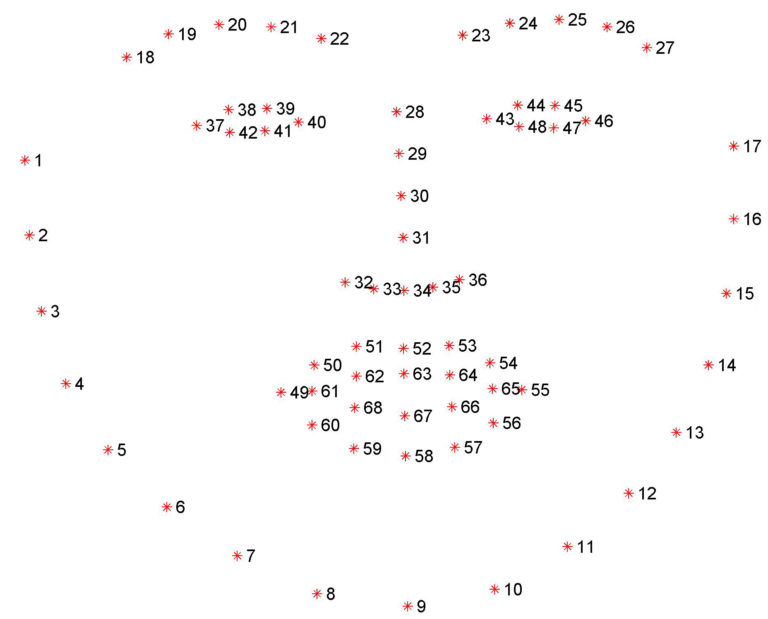
\includegraphics[scale=0.25]{facia_landmarks.jpg}
        \caption{Visualizing the 68 facial landmark coordinates from the iBUG 300-W dataset}
        \label{Landmark}
    \end{figure}
    
    However, for the Project final phase, the predictor will be trained with images coming from the Helen$^{[3]}$ dataset with a 194 points model, which we expect better results.
    
    \begin{figure}[!ht]
    \centering
    \begin{subfigure}{.4\textwidth}
        \centering
        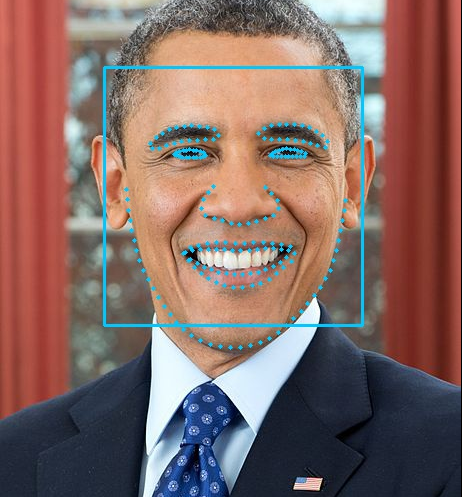
\includegraphics[width=.7\linewidth]{Obama_194.png}
        \caption{194 landmark coordinates}
        \label{fig:sub1}
    \end{subfigure}
    \begin{subfigure}{.4\textwidth}
        \centering
        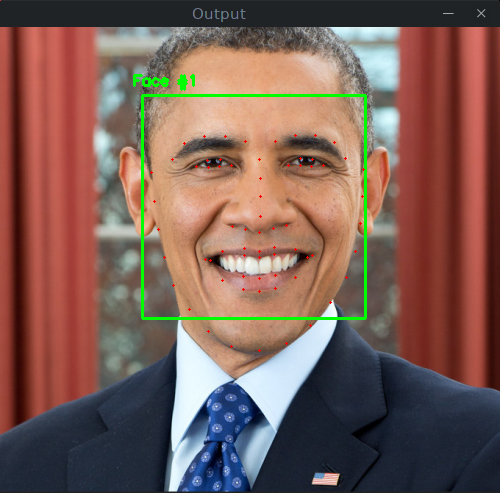
\includegraphics[width=.7\linewidth]{Obama_8.png}
        \caption{68 landmark coordinates}
        \label{fig:sub2}
    \end{subfigure}
    \caption{Comparision between the 194(a) and 68(b) coordinates model}
    \label{fig:test}
    \end{figure}
    
    To train the predictor with the Helen dataset, first we got the annotations file included in the dataset and reorganized it in a xml format. Then new labels were added to the landmarks around the eyes, mouth, nose and eyebrows. The landmarks and labels were adjusted with dlib's imglab tool, included with dlib. Finally the predictor may be be trained with those 194 points and five labels. The training command is as follows:

    \begin{center}
        \large python train\_shape\_predictor.py - -training-file {\it file}  - -test-file {\it file}
    \end{center}
    
    This will generate a predictor.dat file which is the trained predictor data to be used with facial recognition.
    Now, the user may feed the predictor to the application with an image and the program should return a bounding box in each identified objects (face, nose, mouth, eyes, eyebrow). In order to remove the red eyes, all the pixels of the eyes boxes will be traversed in order to check the intensity of their red tones. If the red channel value is much higher when compared to the blue and green channels, then we probably have a red eye there. If this is detected, we just normalize the red value to the blue and green levels, and thus remove the red eyes.\\
    To apply the temperature filter, we will just rise the intensity of the red tones of an image if the user chooses to make the image hotter, or blue tones to make it colder. \\
    Finally, the other filters (gamma and sharpening) will be applied the same way they used in classes assignments but in colored images. To do this, we will converet from RGB space to HSV and apply the filter in the Value channel since they only need to work with contrast, and not color directly.\\
    The key feature replacement will be just a replacement of the identified object by one of the defaults and some smooth filtering/equalisation shall be applied to smooth out the contours.
    
    
\newpage  
\section{First Results}

    Using the pre-trained predictor, we were already able to get a raster around each face identified in the input image and we can manipulate them already. The program can handle RGB and grayscale images, rotated faces and multiple faces in the same image.\\
    The images below show exemples of our first results:
    
    \begin{figure}[!hb]
        \centering
        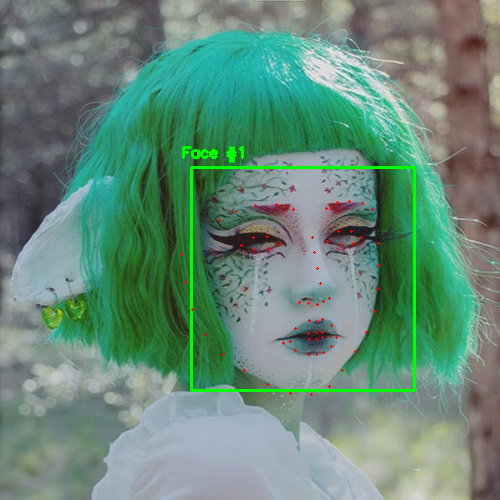
\includegraphics[scale=0.5]{anzusc.png}
        \caption{Example of a facial recognition performed in a colorful image}
        \label{Anzu}
    \end{figure}

    \begin{figure}[!hb]
        \centering
        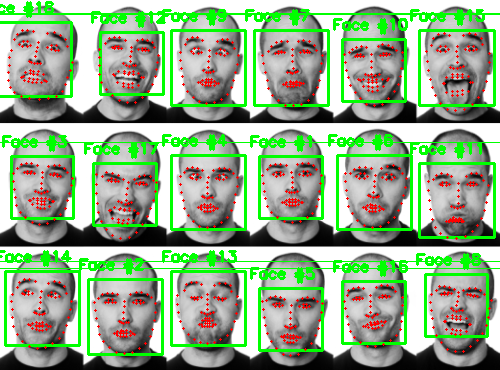
\includegraphics[scale=0.5]{multiple-faces.png}
        \caption{Example of a multiple facial recognition performed in a grayscale image}
        \label{Gray}
    \end{figure}
    
    \begin{figure}[!ht]
        \centering
        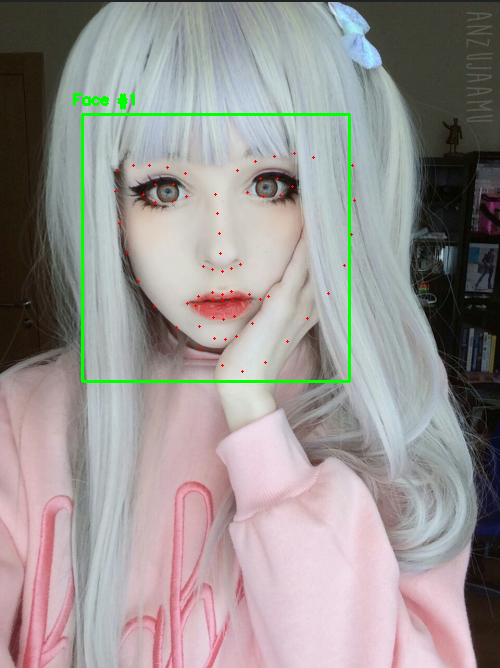
\includegraphics[scale=0.5]{AnzuscWrong.png}
        \caption{Example of a failed recognition that we expect to fix with the 194 point model}
        \label{Anzu2}
    \end{figure}
    
    \footnote{Figure 1: http://www.pyimagesearch.com/2017/04/03/facial-landmarks-dlib-opencv-python/}
    \footnote{Figures 3\&5: https://www.facebook.com/apricotjaamu/}
    \footnote{Figures 4: https://br.pinterest.com/amylamps/multiple-images-photography-project/?lp=true}
    
\newpage

\section{Final Results}
    As we didn't manage to construct the database and train the new 194 landmarks model in time, we decided to use cascade classifiers included with OpenCV to find some characteristics, like eyes. This is a lot more limited than what we previously wanted, however it sufficient for testing a lot of the features we envisioned.

\subsection{Filters}

    \begin{figure}[!ht]
        \centering
        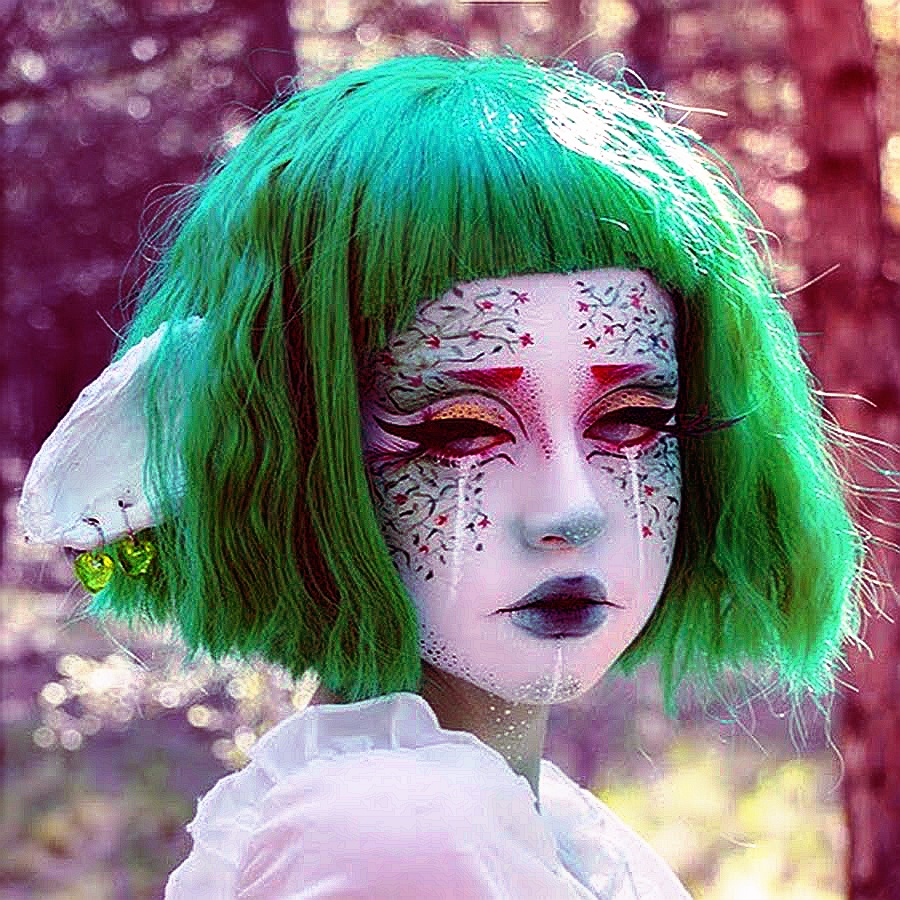
\includegraphics[scale=0.5]{Anzu-test.jpg}
        \caption{Anzu3.jpg after applying Sharpen -> Detail -> Autocontrast -> Equalize filters}
        \label{Anzu-test}
    \end{figure}

\subsection{Distortion}
    For applying distortion, first we transform the image to a grid and then to a mesh-like structure. This facilitates when moving and interpolating points in images. The user may define the grid resolution in X and Y axis separately, and also define the max distortion value, since it will be randomly applied in the image.

    It is possible to obtain interesting effets by tuning the distortion parameters, like a glass or watery effect as seen in~\ref{Anzu-glass} and~\ref{Anzu-watery}

    \begin{figure}[!ht]
        \centering
        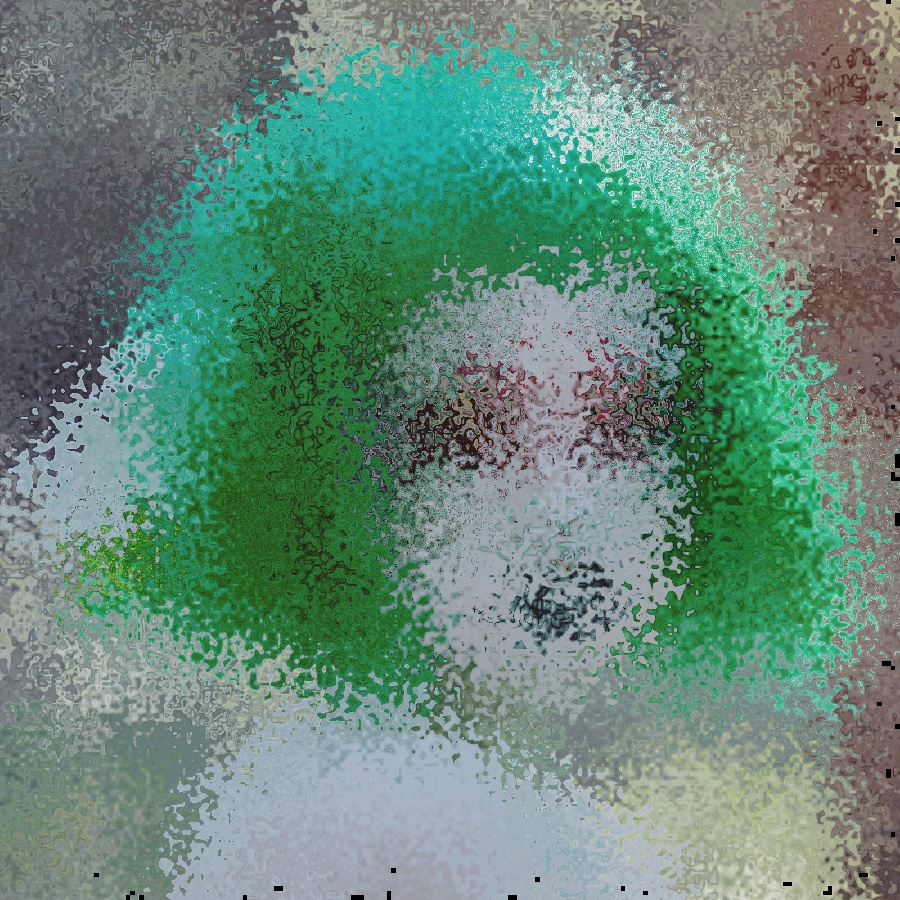
\includegraphics[scale=0.5]{Anzu-glass.jpg}
        \caption{Anzu3.jpg with distortion (x = 200, y = 200, distortion = 50)}
        \label{Anzu-glass}
    \end{figure}

    \begin{figure}[!ht]
        \centering
        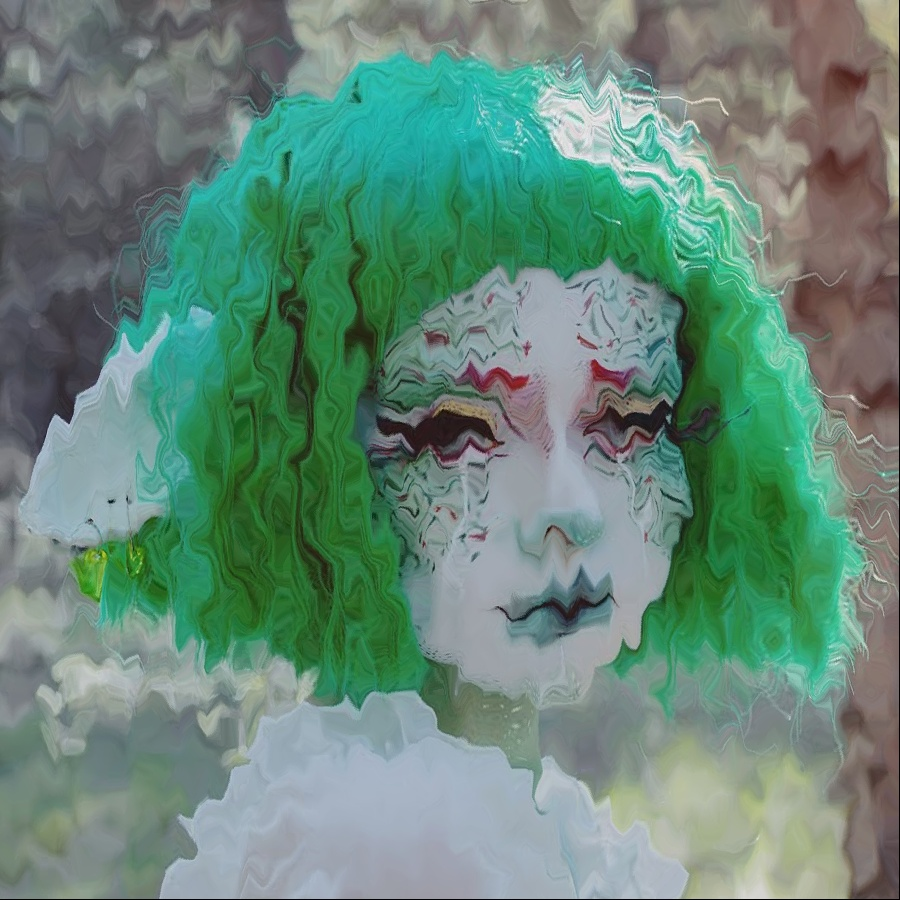
\includegraphics[scale=0.5]{Anzu-watery.jpg}
        \caption{Anzu3.jpg with distortion (x = 65, y = 35, distortion = 15)}
        \label{Anzu-watery}
    \end{figure}

\subsection{Red Eyes}
    For red eyes removel, we used the Haar Cascade Classifier included in OpenCV to locate the eyes. Having the eyes, the program separates the red channel from the green and blue, apply a threshold in the red channel for a minimum red intensity that the user define as possible red eye, apply a closing operation in the image to remove noise and small ``holes'' and finally replace the red pixels with the mean of the green and blue channels. This way, the color seems to blend better with the eye iris.
    The green and blue channels are used as masks when replacing the pixels, to guarantee a smooth eye.

\section{References}

1 - iBUG: ``https://ibug.doc.ic.ac.uk/resources/facial-point-annotations/''\\
\par 2 - Dlib: ``http://dlib.net/imaging.html''\\
\par 3 - Helen: ``http://www.ifp.illinois.edu/~vuongle2/helen/'' \\
\par 4 - Pillow: ``https://python-pillow.org/'' \\
\par 5 - Cascade classifiers: ``https://en.wikipedia.org/wiki/Cascading_classifiers'' \\
\par 6 - OpenCV: ``http://opencv.org/'' \\
\par 7 - Haar Cascades OpenCV: ``http://docs.opencv.org/trunk/d7/d8b/tutorial_py_face_detection.html'' \\

\par 8 - Red eyes removal: ``https://pytech-solution.blogspot.com.br/2017/04/red-eye-correction-from-image-using.html'' \\ % FIXME: Mantem essa referencia?
\par 7 - : ``'' \\


\end{document}
